\documentclass[aspectratio=169]{beamer}
\usepackage[utf8]{inputenc}
\usepackage[T1]{fontenc}
\usepackage{tikz}
\usetikzlibrary{shapes,arrows,positioning,calc,decorations.pathreplacing}

% Couleurs
\definecolor{inputcolor}{RGB}{52, 152, 219}
\definecolor{hiddencolor}{RGB}{39, 174, 96}
\definecolor{outputcolor}{RGB}{231, 76, 60}
\definecolor{grucolor}{RGB}{155, 89, 182}
\definecolor{svmcolor}{RGB}{241, 196, 15}

\begin{document}

% ============================================================================
% SLIDE: MLP Architecture
% ============================================================================
\begin{frame}{MLP Architecture - Multi-Layer Perceptron}
    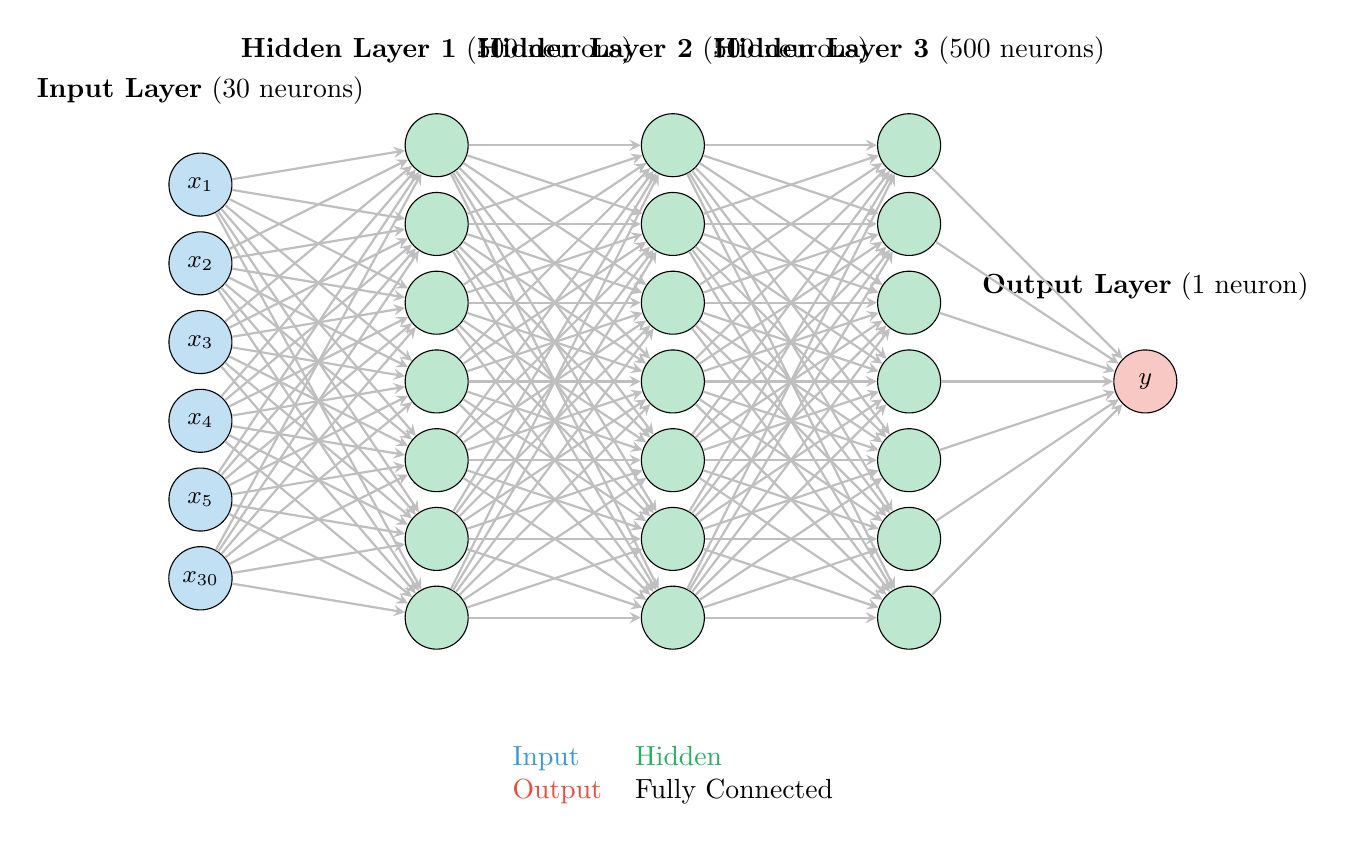
\begin{tikzpicture}[
        node distance=1.5cm and 2cm,
        neuron/.style={circle, draw, minimum size=0.8cm, font=\small},
        layer/.style={rectangle, draw, minimum width=2cm, minimum height=6cm, fill=gray!10},
        arrow/.style={->, >=stealth, thick}
    ]
        
        % Input Layer
        \node[neuron, fill=inputcolor!30] (i1) at (0,2.5) {$x_1$};
        \node[neuron, fill=inputcolor!30] (i2) at (0,1.5) {$x_2$};
        \node[neuron, fill=inputcolor!30] (i3) at (0,0.5) {$x_3$};
        \node[neuron, fill=inputcolor!30] (i4) at (0,-0.5) {$x_4$};
        \node[neuron, fill=inputcolor!30] (i5) at (0,-1.5) {$x_5$};
        \node[neuron, fill=inputcolor!30] (i6) at (0,-2.5) {$x_{30}$};
        \node[above of=i1, yshift=-0.3cm] {\textbf{Input Layer} (30 neurons)};
        
        % Hidden Layer 1
        \node[neuron, fill=hiddencolor!30] (h1_1) at (3,3) {};
        \node[neuron, fill=hiddencolor!30] (h1_2) at (3,2) {};
        \node[neuron, fill=hiddencolor!30] (h1_3) at (3,1) {};
        \node[neuron, fill=hiddencolor!30] (h1_4) at (3,0) {};
        \node[neuron, fill=hiddencolor!30] (h1_5) at (3,-1) {};
        \node[neuron, fill=hiddencolor!30] (h1_6) at (3,-2) {};
        \node[neuron, fill=hiddencolor!30] (h1_7) at (3,-3) {};
        \node[above of=h1_1, yshift=-0.3cm] {\textbf{Hidden Layer 1} (500 neurons)};
        
        % Hidden Layer 2
        \node[neuron, fill=hiddencolor!30] (h2_1) at (6,3) {};
        \node[neuron, fill=hiddencolor!30] (h2_2) at (6,2) {};
        \node[neuron, fill=hiddencolor!30] (h2_3) at (6,1) {};
        \node[neuron, fill=hiddencolor!30] (h2_4) at (6,0) {};
        \node[neuron, fill=hiddencolor!30] (h2_5) at (6,-1) {};
        \node[neuron, fill=hiddencolor!30] (h2_6) at (6,-2) {};
        \node[neuron, fill=hiddencolor!30] (h2_7) at (6,-3) {};
        \node[above of=h2_1, yshift=-0.3cm] {\textbf{Hidden Layer 2} (500 neurons)};
        
        % Hidden Layer 3
        \node[neuron, fill=hiddencolor!30] (h3_1) at (9,3) {};
        \node[neuron, fill=hiddencolor!30] (h3_2) at (9,2) {};
        \node[neuron, fill=hiddencolor!30] (h3_3) at (9,1) {};
        \node[neuron, fill=hiddencolor!30] (h3_4) at (9,0) {};
        \node[neuron, fill=hiddencolor!30] (h3_5) at (9,-1) {};
        \node[neuron, fill=hiddencolor!30] (h3_6) at (9,-2) {};
        \node[neuron, fill=hiddencolor!30] (h3_7) at (9,-3) {};
        \node[above of=h3_1, yshift=-0.3cm] {\textbf{Hidden Layer 3} (500 neurons)};
        
        % Output Layer
        \node[neuron, fill=outputcolor!30] (o1) at (12,0) {$y$};
        \node[above of=o1, yshift=-0.3cm] {\textbf{Output Layer} (1 neuron)};
        
        % Connections Input -> Hidden 1
        \foreach \i in {1,2,3,4,5,6} {
            \foreach \j in {1,2,3,4,5,6,7} {
                \draw[arrow, gray!50] (i\i) -- (h1_\j);
            }
        }
        
        % Connections Hidden 1 -> Hidden 2
        \foreach \i in {1,2,3,4,5,6,7} {
            \foreach \j in {1,2,3,4,5,6,7} {
                \draw[arrow, gray!50] (h1_\i) -- (h2_\j);
            }
        }
        
        % Connections Hidden 2 -> Hidden 3
        \foreach \i in {1,2,3,4,5,6,7} {
            \foreach \j in {1,2,3,4,5,6,7} {
                \draw[arrow, gray!50] (h2_\i) -- (h3_\j);
            }
        }
        
        % Connections Hidden 3 -> Output
        \foreach \i in {1,2,3,4,5,6,7} {
            \draw[arrow, gray!50] (h3_\i) -- (o1);
        }
        
        % Legend
        \node[below of=i6, yshift=-1cm, xshift=6cm] {
            \begin{tabular}{ll}
                \textcolor{inputcolor}{Input} & \textcolor{hiddencolor}{Hidden} \\
                \textcolor{outputcolor}{Output} & Fully Connected
            \end{tabular}
        };
        
    \end{tikzpicture}
    
    \vspace{0.5cm}
    \begin{block}{Architecture}
        \textbf{Paper:} (500, 500, 500) - 30 $\rightarrow$ 500 $\rightarrow$ 500 $\rightarrow$ 500 $\rightarrow$ 1 \\
        \textbf{Notre:} Optimisée - Architecture adaptée selon grid search
    \end{block}
\end{frame}

% ============================================================================
% SLIDE: GRU-SVM Architecture - Part 1: GRU
% ============================================================================
\begin{frame}{GRU-SVM Architecture - Part 1: GRU Layer}
    \begin{tikzpicture}[
        node distance=1cm and 1.5cm,
        neuron/.style={circle, draw, minimum size=0.6cm, font=\tiny},
        grucell/.style={rectangle, draw, minimum width=1.5cm, minimum height=2cm, fill=grucolor!20},
        arrow/.style={->, >=stealth, thick}
    ]
        
        % Input sequence
        \node[neuron, fill=inputcolor!30] (x1) at (0,2) {$x_1$};
        \node[neuron, fill=inputcolor!30] (x2) at (0,1) {$x_2$};
        \node[neuron, fill=inputcolor!30] (x3) at (0,0) {$x_3$};
        \node[neuron, fill=inputcolor!30] (x4) at (0,-1) {$x_{30}$};
        \node[left of=x2, xshift=-0.5cm] {\textbf{Input Features} (30)};
        
        % GRU Cells (simplified - showing 3 out of 48)
        \node[grucell] (gru1) at (3,1.5) {\textbf{GRU} \\ Unit 1};
        \node[grucell] (gru2) at (5,1.5) {\textbf{GRU} \\ Unit 2};
        \node[grucell] (gru3) at (7,1.5) {\textbf{GRU} \\ Unit ...};
        \node[grucell] (gru48) at (9,1.5) {\textbf{GRU} \\ Unit 48};
        
        % Connections to GRU
        \foreach \i in {1,2,3,4} {
            \draw[arrow, gray!50] (x\i) -- (gru1);
        }
        
        % GRU internal connections (recurrent)
        \draw[arrow, grucolor, thick] (gru1) -- node[above, font=\tiny] {$h_1$} (gru2);
        \draw[arrow, grucolor, thick] (gru2) -- node[above, font=\tiny] {$h_2$} (gru3);
        \draw[arrow, grucolor, dashed] (gru3) -- (gru48);
        
        % GRU output
        \node[neuron, fill=grucolor!30] (h_out) at (11.5,1.5) {$h$};
        \draw[arrow, grucolor, thick] (gru48) -- (h_out);
        
        % Dropout
        \node[rectangle, draw, fill=gray!20, minimum width=1cm, minimum height=0.5cm] (drop1) at (13,1.5) {Dropout 0.5};
        \draw[arrow] (h_out) -- (drop1);
        
        % BatchNorm
        \node[rectangle, draw, fill=gray!20, minimum width=1cm, minimum height=0.5cm] (bn1) at (15,1.5) {BatchNorm};
        \draw[arrow] (drop1) -- (bn1);
        
        % Dense layer
        \node[neuron, fill=hiddencolor!30] (d1) at (17,2) {};
        \node[neuron, fill=hiddencolor!30] (d2) at (17,1) {};
        \node[neuron, fill=hiddencolor!30] (d3) at (17,0) {};
        \node[above of=d1, yshift=-0.2cm, font=\tiny] {\textbf{Dense} (24)};
        \draw[arrow] (bn1) -- (d1);
        \draw[arrow] (bn1) -- (d2);
        \draw[arrow] (bn1) -- (d3);
        
        % Dropout 2
        \node[rectangle, draw, fill=gray!20, minimum width=1cm, minimum height=0.5cm] (drop2) at (19,1) {Dropout 0.4};
        \draw[arrow] (d2) -- (drop2);
        
        % BatchNorm 2
        \node[rectangle, draw, fill=gray!20, minimum width=1cm, minimum height=0.5cm] (bn2) at (21,1) {BatchNorm};
        \draw[arrow] (drop2) -- (bn2);
        
        % Output
        \node[neuron, fill=outputcolor!30] (out) at (23,1) {$y$};
        \draw[arrow] (bn2) -- (out);
        
        % Labels
        \node[below of=gru1, yshift=0.5cm, font=\tiny] {\textbf{Paper:} 128 units};
        \node[below of=gru48, yshift=0.5cm, font=\tiny, text color=ourgreen] {\textbf{Notre:} 48 units};
        
    \end{tikzpicture}
    
    \vspace{0.3cm}
    \begin{block}{GRU Architecture Comparison}
        \textbf{Paper:} Input(30) $\rightarrow$ GRU(128) $\rightarrow$ Dropout(0.3) $\rightarrow$ Dense(32) $\rightarrow$ Dropout(0.5) $\rightarrow$ Output(1) \\
        \textbf{Notre:} Input(30) $\rightarrow$ GRU(48)+L2 $\rightarrow$ Dropout(0.5) $\rightarrow$ BatchNorm $\rightarrow$ Dense(24)+L2 $\rightarrow$ Dropout(0.4) $\rightarrow$ BatchNorm $\rightarrow$ Output(1)
    \end{block}
\end{frame}

% ============================================================================
% SLIDE: GRU-SVM Architecture - Complete
% ============================================================================
\begin{frame}{GRU-SVM Architecture - Complete Hybrid Model}
    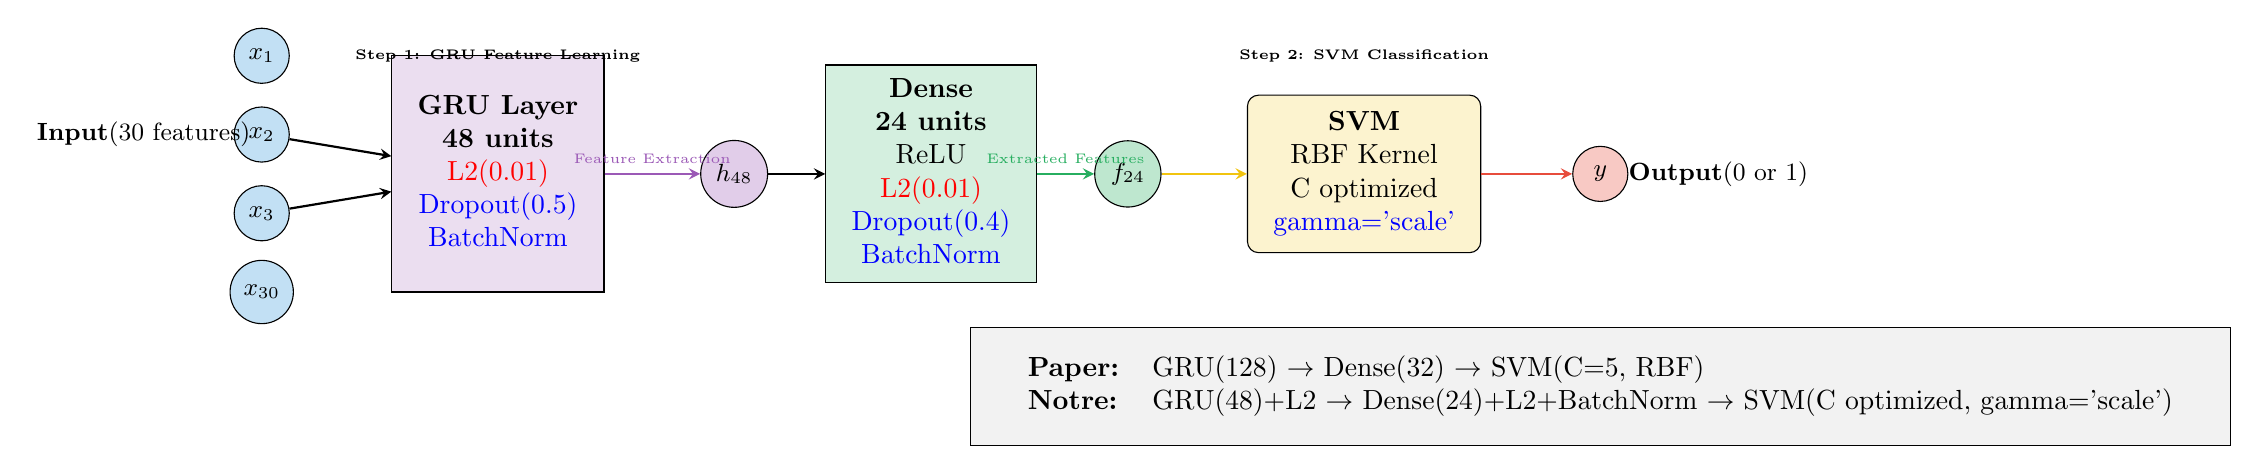
\begin{tikzpicture}[
        node distance=1.2cm and 2cm,
        neuron/.style={circle, draw, minimum size=0.7cm, font=\small},
        grucell/.style={rectangle, draw, minimum width=2cm, minimum height=3cm, fill=grucolor!20},
        svm/.style={rectangle, draw, minimum width=2cm, minimum height=2cm, fill=svmcolor!20, rounded corners},
        arrow/.style={->, >=stealth, thick},
        dashedarrow/.style={->, >=stealth, thick, dashed}
    ]
        
        % Input
        \node[neuron, fill=inputcolor!30] (x1) at (0,1.5) {$x_1$};
        \node[neuron, fill=inputcolor!30] (x2) at (0,0.5) {$x_2$};
        \node[neuron, fill=inputcolor!30] (x3) at (0,-0.5) {$x_3$};
        \node[neuron, fill=inputcolor!30] (x4) at (0,-1.5) {$x_{30}$};
        \node[left of=x2, xshift=-0.3cm, font=\small] {\textbf{Input} \\ (30 features)};
        
        % GRU Block
        \node[grucell] (gru_block) at (3,0) {
            \begin{tabular}{c}
                \textbf{GRU Layer} \\
                \textbf{48 units} \\
                \textcolor{red}{L2(0.01)} \\
                \textcolor{blue}{Dropout(0.5)} \\
                \textcolor{blue}{BatchNorm}
            \end{tabular}
        };
        \draw[arrow] (x2) -- (gru_block);
        \draw[arrow] (x3) -- (gru_block);
        
        % GRU Output (hidden state)
        \node[neuron, fill=grucolor!30] (h_gru) at (6,0) {$h_{48}$};
        \draw[arrow, grucolor] (gru_block) -- node[above, font=\tiny] {Feature Extraction} (h_gru);
        
        % Dense Layer
        \node[rectangle, draw, minimum width=1.5cm, minimum height=2cm, fill=hiddencolor!20] (dense) at (8.5,0) {
            \begin{tabular}{c}
                \textbf{Dense} \\
                \textbf{24 units} \\
                ReLU \\
                \textcolor{red}{L2(0.01)} \\
                \textcolor{blue}{Dropout(0.4)} \\
                \textcolor{blue}{BatchNorm}
            \end{tabular}
        };
        \draw[arrow] (h_gru) -- (dense);
        
        % Feature Extractor Output (for SVM)
        \node[neuron, fill=hiddencolor!30] (features) at (11,0) {$f_{24}$};
        \draw[arrow, hiddencolor] (dense) -- node[above, font=\tiny] {Extracted Features} (features);
        
        % SVM Block
        \node[svm] (svm_block) at (14,0) {
            \begin{tabular}{c}
                \textbf{SVM} \\
                RBF Kernel \\
                C optimized \\
                \textcolor{blue}{gamma='scale'}
            \end{tabular}
        };
        \draw[arrow, svmcolor, thick] (features) -- (svm_block);
        
        % Final Output
        \node[neuron, fill=outputcolor!30] (output) at (17,0) {$y$};
        \draw[arrow, outputcolor, thick] (svm_block) -- (output);
        \node[right of=output, xshift=0.3cm, font=\small] {\textbf{Output} \\ (0 or 1)};
        
        % Labels and annotations
        \node[above of=gru_block, yshift=0.3cm, font=\tiny] {\textbf{Step 1: GRU Feature Learning}};
        \node[above of=svm_block, yshift=0.3cm, font=\tiny] {\textbf{Step 2: SVM Classification}};
        
        % Comparison box
        \node[rectangle, draw, fill=gray!10, minimum width=16cm, minimum height=1.5cm, 
              below of=output, yshift=-1.5cm] (comparison) {
            \begin{tabular}{ll}
                \textbf{Paper:} & GRU(128) $\rightarrow$ Dense(32) $\rightarrow$ SVM(C=5, RBF) \\
                \textbf{Notre:} & GRU(48)+L2 $\rightarrow$ Dense(24)+L2+BatchNorm $\rightarrow$ SVM(C optimized, gamma='scale')
            \end{tabular}
        };
        
    \end{tikzpicture}
    
    \vspace{0.2cm}
    \begin{alertblock}{Architecture Hybride}
        Le modèle GRU-SVM combine l'apprentissage de features profondes (GRU) avec la classification robuste (SVM)
    \end{alertblock}
\end{frame}

% ============================================================================
% SLIDE: GRU Cell Detailed Structure
% ============================================================================
\begin{frame}{GRU Cell - Detailed Internal Structure}
    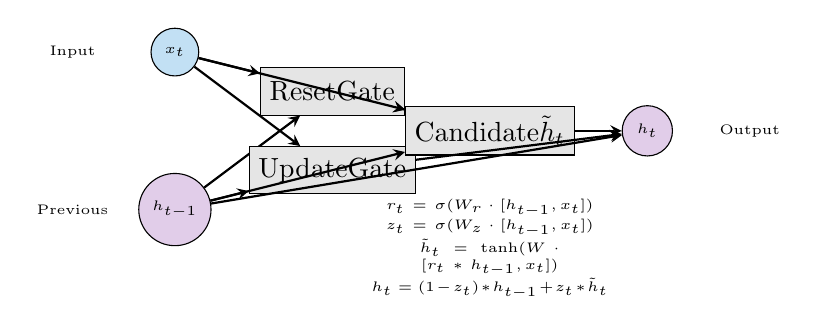
\begin{tikzpicture}[
        node distance=1cm,
        neuron/.style={circle, draw, minimum size=0.5cm, font=\tiny},
        gate/.style={rectangle, draw, minimum width=1cm, minimum height=0.6cm, fill=gray!20},
        arrow/.style={->, >=stealth, thick}
    ]
        
        % Input
        \node[neuron, fill=inputcolor!30] (x_t) at (0,2) {$x_t$};
        \node[left of=x_t, xshift=-0.3cm, font=\tiny] {Input};
        
        % Previous hidden state
        \node[neuron, fill=grucolor!30] (h_prev) at (0,0) {$h_{t-1}$};
        \node[left of=h_prev, xshift=-0.3cm, font=\tiny] {Previous};
        
        % Reset gate
        \node[gate] (r_gate) at (2,1.5) {Reset \\ Gate};
        \draw[arrow] (x_t) -- (r_gate);
        \draw[arrow] (h_prev) -- (r_gate);
        
        % Update gate
        \node[gate] (z_gate) at (2,0.5) {Update \\ Gate};
        \draw[arrow] (x_t) -- (z_gate);
        \draw[arrow] (h_prev) -- (z_gate);
        
        % Candidate activation
        \node[gate] (h_candidate) at (4,1) {Candidate \\ $\tilde{h}_t$};
        \draw[arrow] (x_t) -- (h_candidate);
        \draw[arrow] (r_gate) -- (h_candidate);
        \draw[arrow] (h_prev) -- (h_candidate);
        
        % New hidden state
        \node[neuron, fill=grucolor!30] (h_t) at (6,1) {$h_t$};
        \draw[arrow] (h_candidate) -- (h_t);
        \draw[arrow] (z_gate) -- (h_t);
        \draw[arrow] (h_prev) -- (h_t);
        
        % Output
        \node[right of=h_t, xshift=0.3cm, font=\tiny] {Output};
        
        % Formula annotations
        \node[below of=h_candidate, yshift=-0.5cm, font=\tiny, text width=3cm, align=center] {
            $r_t = \sigma(W_r \cdot [h_{t-1}, x_t])$ \\
            $z_t = \sigma(W_z \cdot [h_{t-1}, x_t])$ \\
            $\tilde{h}_t = \tanh(W \cdot [r_t * h_{t-1}, x_t])$ \\
            $h_t = (1-z_t) * h_{t-1} + z_t * \tilde{h}_t$
        };
        
    \end{tikzpicture}
    
    \vspace{0.5cm}
    \begin{block}{GRU Cell Operations}
        \textbf{Reset Gate ($r_t$):} Détermine combien d'information passée à oublier \\
        \textbf{Update Gate ($z_t$):} Détermine combien d'information nouvelle à garder \\
        \textbf{Candidate ($\tilde{h}_t$):} Nouvelle information candidate \\
        \textbf{Hidden State ($h_t$):} État caché final (combinaison de l'ancien et du nouveau)
    \end{block}
\end{frame}

% ============================================================================
% SLIDE: MLP vs GRU-SVM Comparison
% ============================================================================
\begin{frame}{MLP vs GRU-SVM - Architecture Comparison}
    \begin{columns}
        \column{0.5\textwidth}
        \begin{block}{MLP Architecture}
            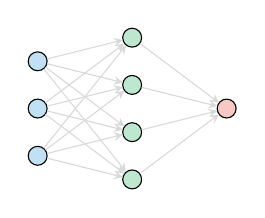
\begin{tikzpicture}[scale=0.6, transform shape,
                neuron/.style={circle, draw, minimum size=0.4cm, font=\tiny},
                arrow/.style={->, >=stealth, thin}]
                
                % Input
                \node[neuron, fill=inputcolor!30] (i1) at (0,1) {};
                \node[neuron, fill=inputcolor!30] (i2) at (0,0) {};
                \node[neuron, fill=inputcolor!30] (i3) at (0,-1) {};
                
                % Hidden
                \node[neuron, fill=hiddencolor!30] (h1) at (2,1.5) {};
                \node[neuron, fill=hiddencolor!30] (h2) at (2,0.5) {};
                \node[neuron, fill=hiddencolor!30] (h3) at (2,-0.5) {};
                \node[neuron, fill=hiddencolor!30] (h4) at (2,-1.5) {};
                
                % Output
                \node[neuron, fill=outputcolor!30] (o1) at (4,0) {};
                
                % Connections
                \foreach \i in {1,2,3} {
                    \foreach \j in {1,2,3,4} {
                        \draw[arrow, gray!30] (i\i) -- (h\j);
                    }
                }
                \foreach \i in {1,2,3,4} {
                    \draw[arrow, gray!30] (h\i) -- (o1);
                }
                
            \end{tikzpicture}
            \begin{itemize}
                \item Fully connected layers
                \item Feedforward only
                \item No memory/sequence
            \end{itemize}
        \end{block}
        
        \column{0.5\textwidth}
        \begin{block}{GRU-SVM Architecture}
            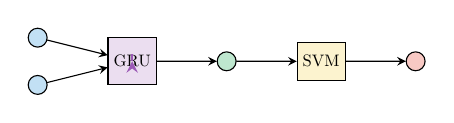
\begin{tikzpicture}[scale=0.6, transform shape,
                neuron/.style={circle, draw, minimum size=0.4cm, font=\tiny},
                gru/.style={rectangle, draw, fill=grucolor!20, minimum width=0.8cm, minimum height=1cm},
                svm/.style={rectangle, draw, fill=svmcolor!20, minimum width=0.8cm, minimum height=0.8cm},
                arrow/.style={->, >=stealth, thin}]
                
                % Input
                \node[neuron, fill=inputcolor!30] (i1) at (0,1) {};
                \node[neuron, fill=inputcolor!30] (i2) at (0,0) {};
                
                % GRU
                \node[gru] (gru) at (2,0.5) {GRU};
                \draw[arrow] (i1) -- (gru);
                \draw[arrow] (i2) -- (gru);
                
                % Recurrent connection
                \draw[arrow, grucolor, thick, bend left=30] (gru) to (gru);
                
                % Dense
                \node[neuron, fill=hiddencolor!30] (d) at (4,0.5) {};
                \draw[arrow] (gru) -- (d);
                
                % SVM
                \node[svm] (svm) at (6,0.5) {SVM};
                \draw[arrow] (d) -- (svm);
                
                % Output
                \node[neuron, fill=outputcolor!30] (o1) at (8,0.5) {};
                \draw[arrow] (svm) -- (o1);
                
            \end{tikzpicture}
            \begin{itemize}
                \item GRU: Sequential processing
                \item Memory/context aware
                \item SVM: Robust classification
            \end{itemize}
        \end{block}
    \end{columns}
    
    \vspace{0.3cm}
    \begin{alertblock}{Différences Clés}
        \textbf{MLP:} Traite toutes les features simultanément, pas de mémoire \\
        \textbf{GRU-SVM:} Traite séquentiellement avec mémoire, puis classification robuste
    \end{alertblock}
\end{frame}

\end{document}

